\section{Registration}

{
\setbeamertemplate{background}{}
\setbeamertemplate{navigation symbols}{}
\setbeamercolor{background canvas}{bg={black}}
\color{white}
\begin{frame}[plain]
\fontsize{36pt}{36pt}\selectfont
\center
\begin{center}
Refactored Registration Framework
\end{center}

\fontsize{12pt}{12pt}\selectfont
\begin{center}
Insight Software Consortium
\end{center}
\vskip12pt
\begin{center}
 PICSL @ University of Pennsylvania 
\end{center}
\vskip12pt
\begin{center}
 Brian Avants, Nicholas Tustison, Gang Song, \\ 
Baohua Wu, Michael Stauffer, James C. Gee
\end{center}
\end{frame}
}

\subsection{Introduction}

\begin{frame}
\frametitle{What is registration?}
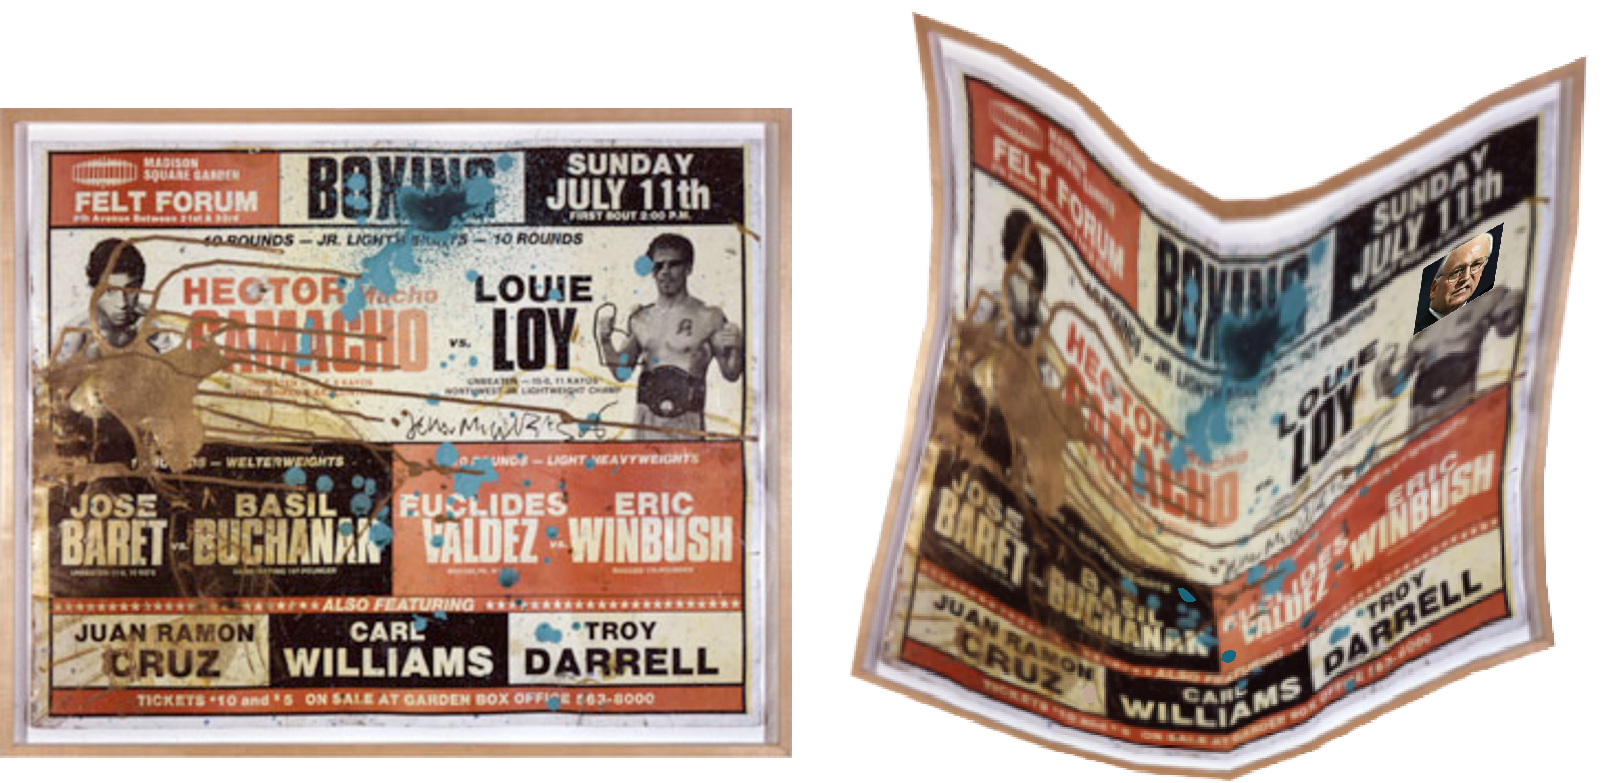
\includegraphics[height=2in]{../Art/RegistrationBasquiatWarp.pdf}
\end{frame}

\begin{frame}
\frametitle{What is registration?}
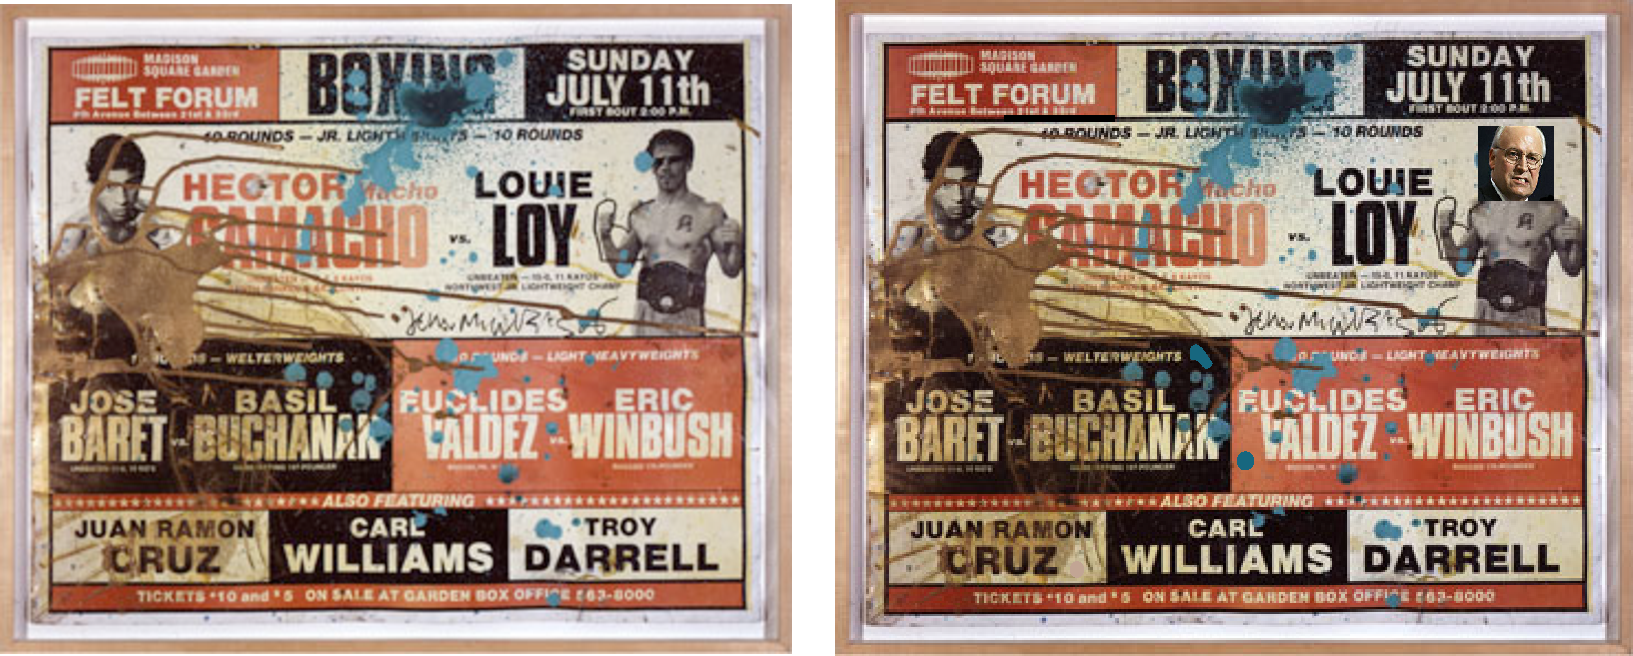
\includegraphics[height=1.8in]{../Art/RegistrationBasquiatDeWarp.pdf}
\vskip20pt
\begin{displaymath}
\| I ( x ) - J(\phi(x)) \|^2  + R(\phi( x))
\end{displaymath}
\end{frame}

 \centeredlargetext{white}{black}{
ITK v3 framework
\vskip20pt
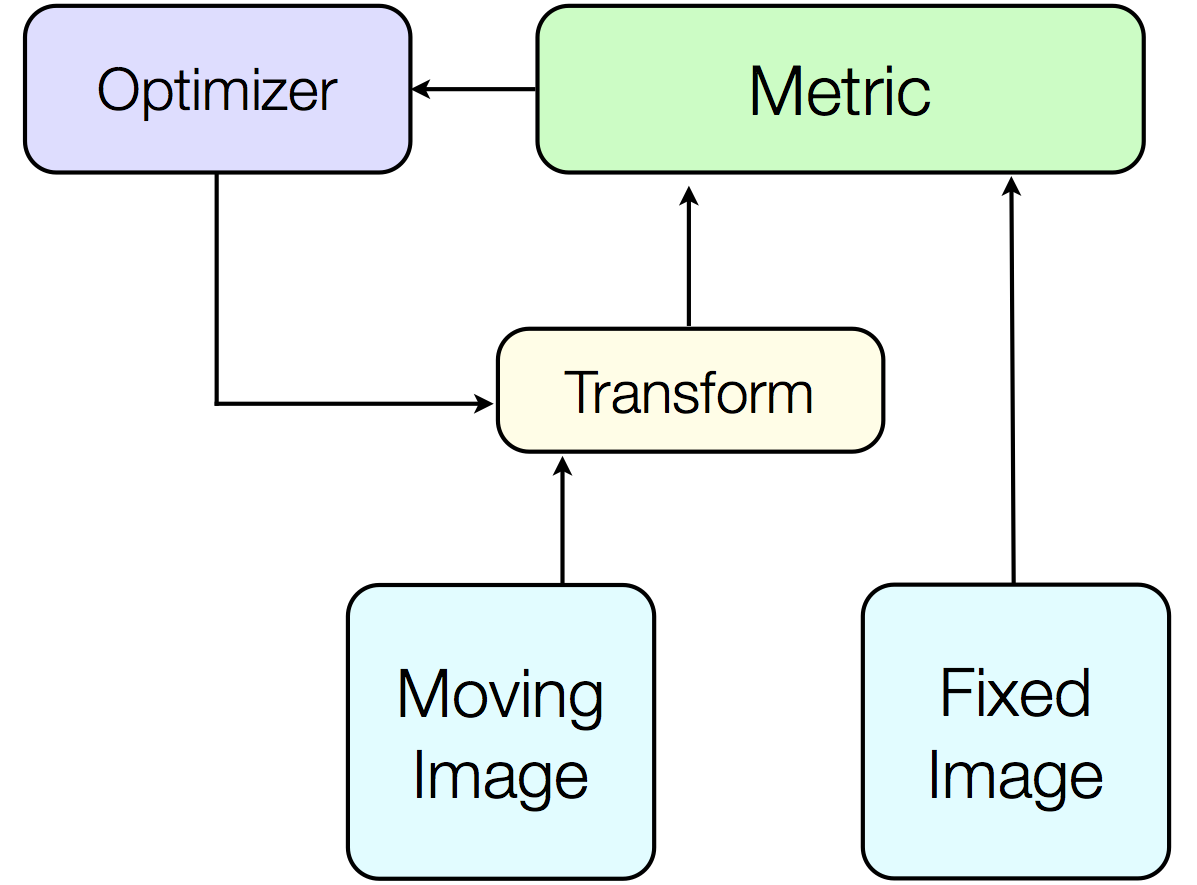
\includegraphics[height=2.2in]{../Art/itkv3reg}
 }

 \centeredlargetext{white}{black}{
ITK v4 framework
\vskip20pt
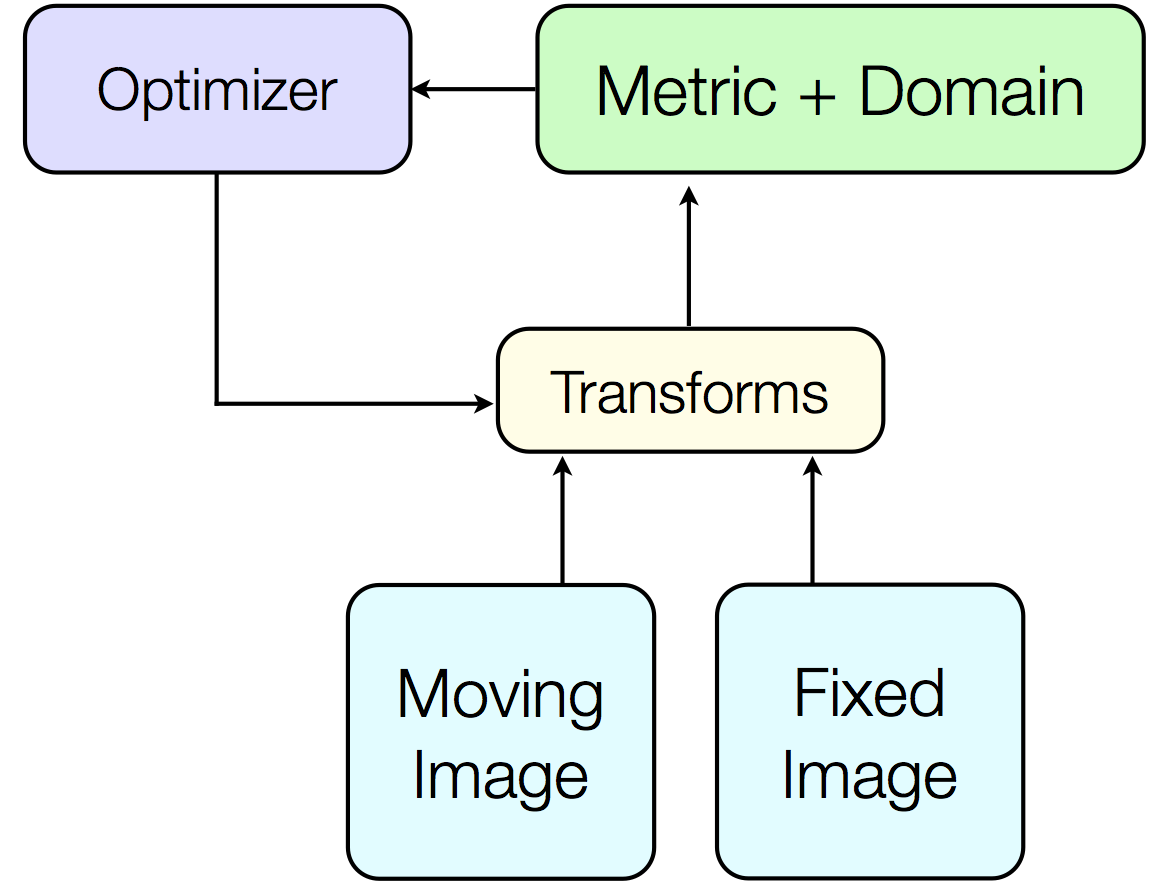
\includegraphics[height=2.2in]{../Art/itkv4reg}
 }

\begin{frame}
\frametitle{Exercise 1: Look at options for a registration program}
\begin{verbatim}
~/bin/ANTS/bin/antsRegistration --help | less
\end{verbatim}
\end{frame}

\begin{frame}
\frametitle{Composite transformations}
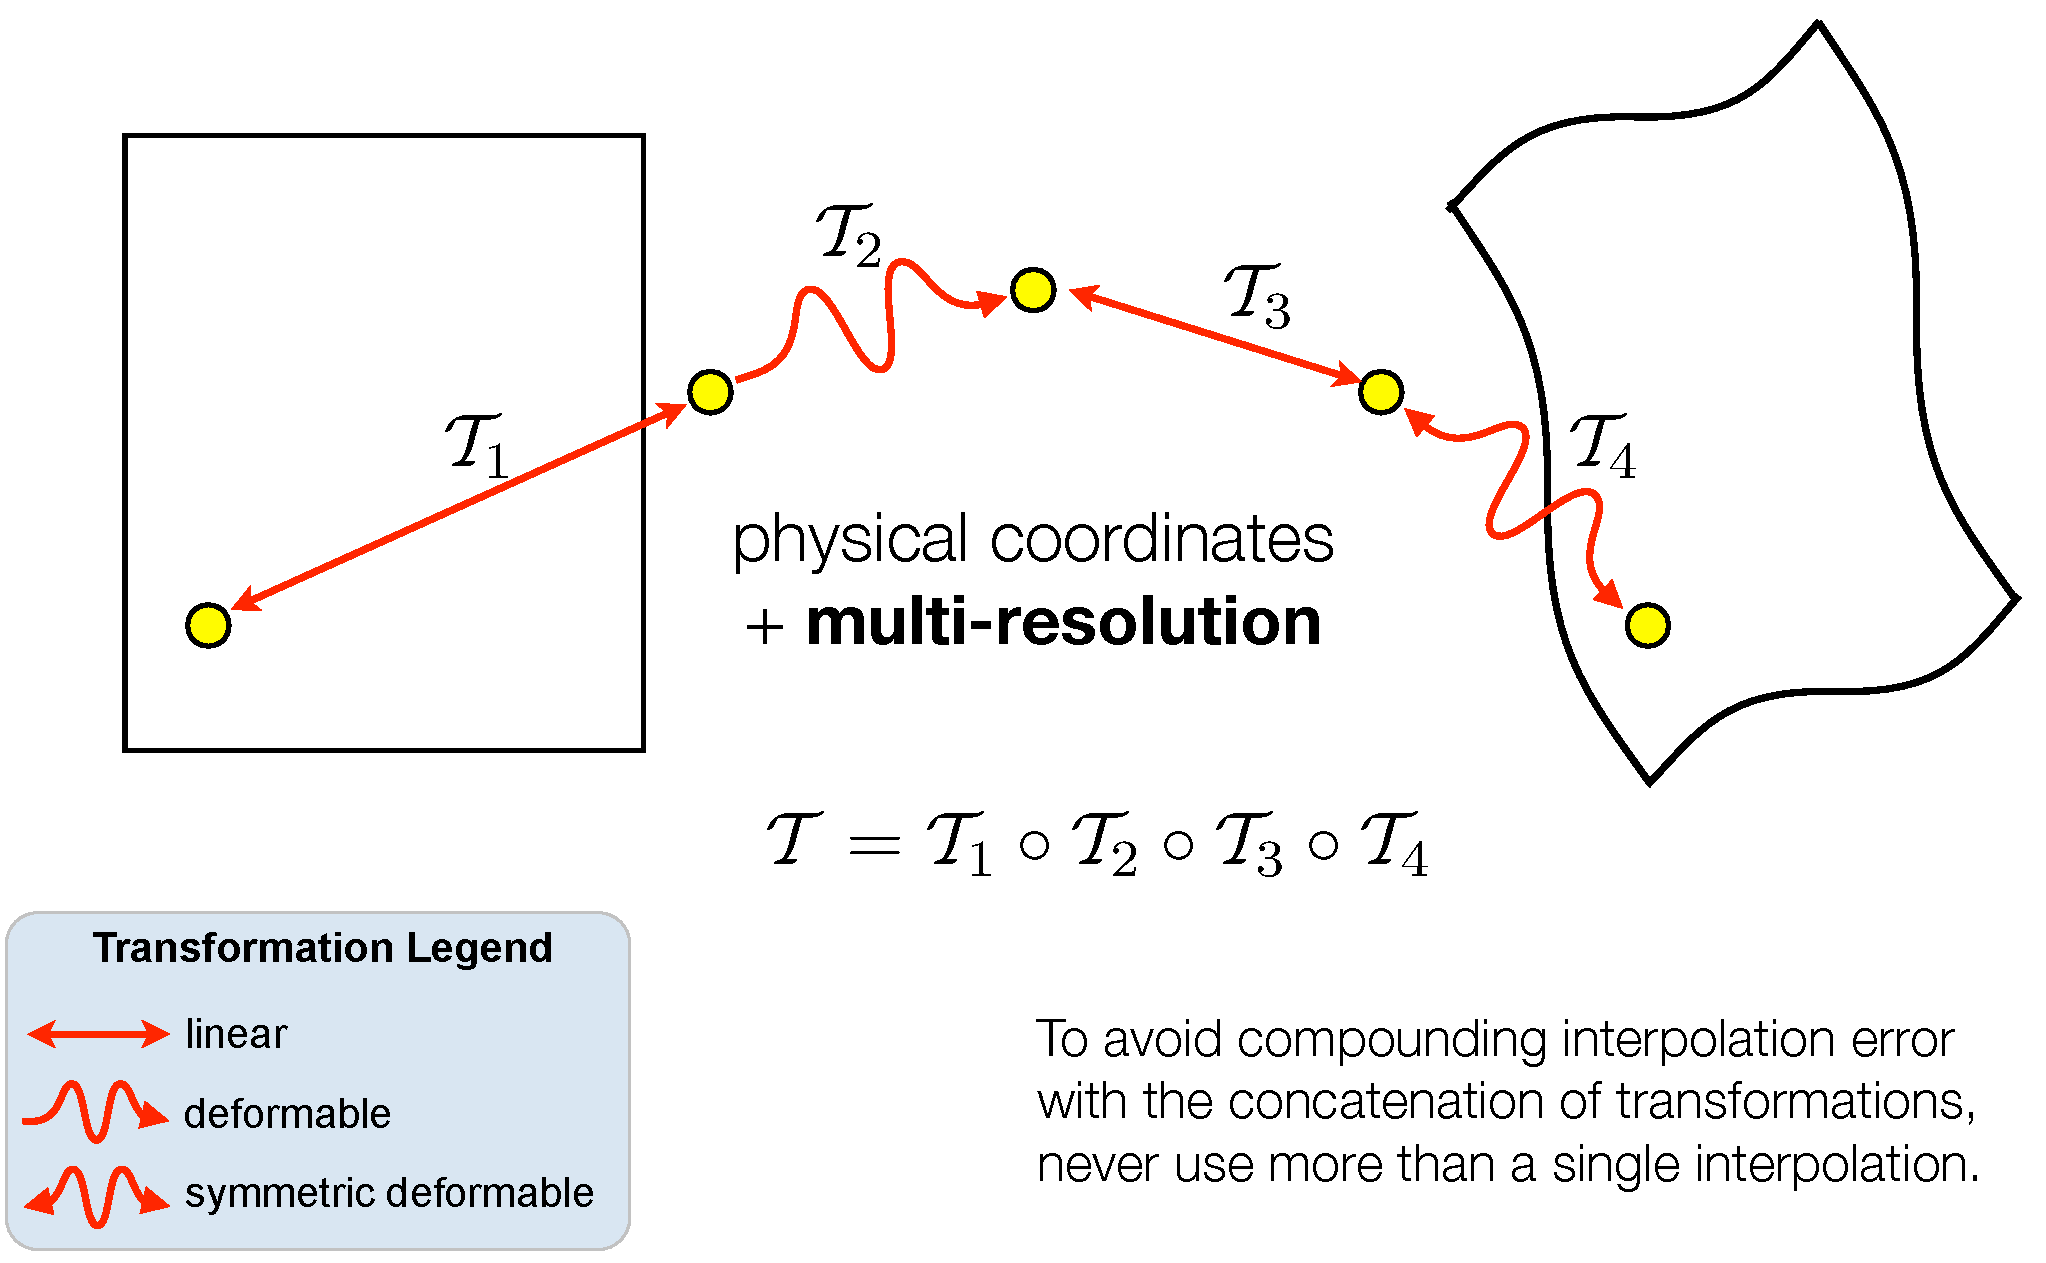
\includegraphics[height=2.5in]{../Art/composite}
\end{frame}

\subsection{Refactoring overview}

\begin{frame}
\frametitle{Image Registration Refactoring}
\Large
\begin{itemize}
\item Unify frameworks: local \& global 
\pause
\item New metrics and transform operations for vectors \&  tensors
\pause
\item Unbiased registration
\pause
\item Multi-threading throughout the metrics
\pause 
\item Automated parameter scaling
\end{itemize}
\end{frame}

\begin{frame}
\frametitle{Unified framework}
\Large
\begin{itemize}
\item Local \& global transforms treated the same in resampler
\item Both types available to (revised) optimizers
\item Revised metrics optimized for these operations
\item Tensors, vector, scalars treated transparently
\end{itemize}
\end{frame}
\subsection{Example}
 \centeredlargetext{white}{black}{
\centering Example Registration
}

\begin{frame}
\frametitle{Image Registration Refactoring: Brain + N-hood CC}
\textcolor{red}{./bin/ITKRegistrationRefactoringTestDriver itkANTSNeighborhoodCorrelationImageToImageObjectRegistrationTest}\\
\textcolor{blue}{r16slice.jpg r64slice.jpg out.nii.gz  50 500 }\\
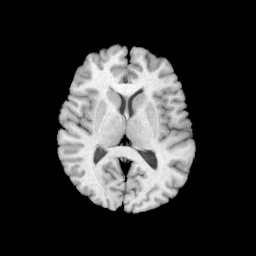
\includegraphics[height=2.2in]{../Art/r16slice.jpg}
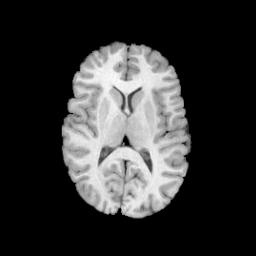
\includegraphics[height=2.2in]{../Art/r64slice.jpg}
\end{frame}

\begin{frame}
\frametitle{Image Registration Code: Brain + N-hood CC}
\begin{itemize}
\item Define the metric
\lstlistingwithnumber{171}{175}{itkANTSNeighborhoodCorrelationImageToImageObjectRegistrationTest.cxx}
\item Define the transforms
\lstlistingwithnumber{165}{168}{itkANTSNeighborhoodCorrelationImageToImageObjectRegistrationTest.cxx}
\lstlistingwithnumber{138}{141}{itkANTSNeighborhoodCorrelationImageToImageObjectRegistrationTest.cxx}
\item Resample the image
\lstlistingwithnumber{201}{202}{itkANTSNeighborhoodCorrelationImageToImageObjectRegistrationTest.cxx}
\end{itemize}

\end{frame}

\begin{frame}
\frametitle{Image Registration Refactoring: Composite Tx + MI}
\textcolor{red}{./bin/ITKRegistrationRefactoringTestDriver itkThevenazMutualInformationImageToImageObjectRegistrationTest }\\
\textcolor{blue}{face\_avg.jpg face\_c.jpg out.nii.gz  50 0.001 0.75 }\\
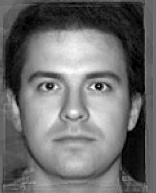
\includegraphics[height=2.2in]{../Art/face_avg.jpg}
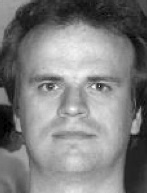
\includegraphics[height=2.2in]{../Art/face_c.jpg}
\end{frame}

\begin{frame}
\frametitle{Image Registration Result: Composite Tx + MI}
\textcolor{red}{./bin/ITKRegistrationRefactoringTestDriver itkThevenazMutualInformationImageToImageObjectRegistrationTest }\\
\textcolor{blue}{face\_avg.jpg face\_c.jpg out.nii.gz  50 0.001 0.75 }\\
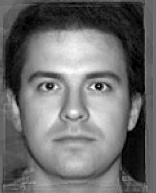
\includegraphics[height=2.2in]{../Art/face_avg.jpg}
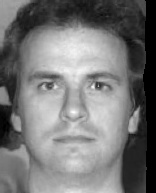
\includegraphics[height=2.2in]{../Art/face_c_to_face_avg.jpg}
\end{frame}

\begin{frame}
\frametitle{Image Registration Code: Composite Tx + MI}
\begin{itemize}
\item Define the metric
\lstlistingwithnumber{186}{189}{itkThevenazMutualInformationImageToImageObjectRegistrationTest.cxx}
\item Estimate scaling parameters for the affine transform
\lstlistingwithnumber{207}{210}{itkThevenazMutualInformationImageToImageObjectRegistrationTest.cxx}
\item Run the affine then add it to composite along with a new
  deformation transform
\lstlistingwithnumber{233}{238}{itkThevenazMutualInformationImageToImageObjectRegistrationTest.cxx}
\end{itemize}
\end{frame}

\begin{frame}
\frametitle{Image Registration Refactoring Example}
\textcolor{red}{./bin/ITKRegistrationRefactoringTestDriver itkThevenazMutualInformationImageToImageObjectRegistrationTest }\\
\textcolor{blue}{face\_avg.jpg face\_b.jpg out.nii.gz  50 0.001 0.75 }\\
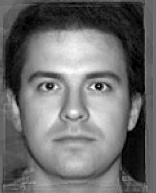
\includegraphics[height=2.2in]{../Art/face_avg.jpg}
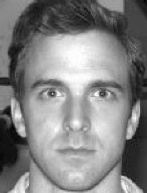
\includegraphics[height=2.2in]{../Art/face_b.jpg}
\end{frame}

\begin{frame}
\frametitle{Image Registration Refactoring Example}
\textcolor{red}{./bin/ITKRegistrationRefactoringTestDriver itkThevenazMutualInformationImageToImageObjectRegistrationTest }\\
\textcolor{blue}{face\_avg.jpg face\_b.jpg out.nii.gz  50 0.001 0.75 }\\
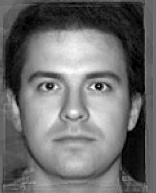
\includegraphics[height=2.2in]{../Art/face_avg.jpg}
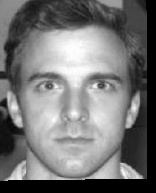
\includegraphics[height=2.2in]{../Art/face_b_to_face_avg_aff.jpg}
\end{frame}
\begin{frame}
\frametitle{Image Registration Refactoring Example}
\textcolor{red}{./bin/ITKRegistrationRefactoringTestDriver itkThevenazMutualInformationImageToImageObjectRegistrationTest }\\
\textcolor{blue}{face\_avg.jpg face\_b.jpg out.nii.gz  50 0.001 0.75 }\\
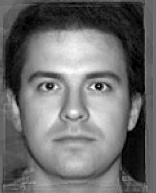
\includegraphics[height=2.2in]{../Art/face_avg.jpg}
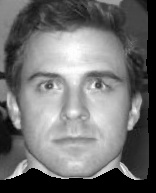
\includegraphics[height=2.2in]{../Art/face_b_to_face_avg.jpg}
\vskip12pt
25 seconds (1 thread) vs 16 seconds (2 threads) on Macbook Air.
\end{frame}

\begin{frame}
\frametitle{Image Registration Refactoring Example}
\textcolor{red}{./bin/ITKRegistrationRefactoringTestDriver itkThevenazMutualInformationImageToImageObjectRegistrationTest }\\
\textcolor{blue}{r16slice.jpg r64slice\_neg.jpg out.nii.gz  50 0.001 0.75 }\\
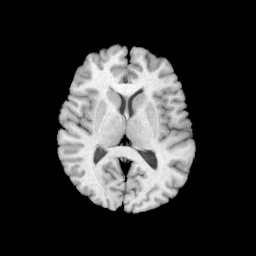
\includegraphics[height=2.2in]{../Art/r16slice.jpg}
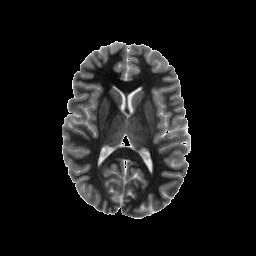
\includegraphics[height=2.2in]{../Art/r64slice_neg.jpg}
\end{frame}

\begin{frame}
\frametitle{Image Registration Refactoring Example}
\textcolor{red}{./bin/ITKRegistrationRefactoringTestDriver itkThevenazMutualInformationImageToImageObjectRegistrationTest }\\
\textcolor{blue}{r16slice.jpg r64slice\_neg.jpg out.nii.gz  50 0.001 0.75 }\\
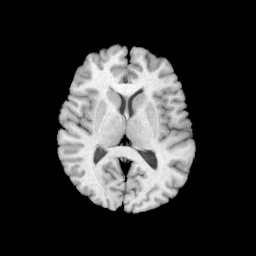
\includegraphics[height=2.2in]{../Art/r16slice.jpg}
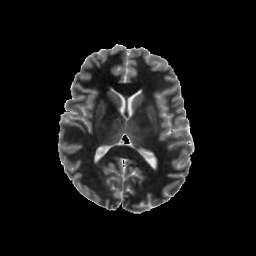
\includegraphics[height=2.2in]{../Art/r64slice_neg_to_16.jpg}
\end{frame}
